\documentclass[12pt,]{article}
\usepackage{lmodern}
\usepackage{amssymb,amsmath}
\usepackage{ifxetex,ifluatex}
\usepackage{fixltx2e} % provides \textsubscript
\ifnum 0\ifxetex 1\fi\ifluatex 1\fi=0 % if pdftex
  \usepackage[T1]{fontenc}
  \usepackage[utf8]{inputenc}
\else % if luatex or xelatex
  \ifxetex
    \usepackage{mathspec}
  \else
    \usepackage{fontspec}
  \fi
  \defaultfontfeatures{Ligatures=TeX,Scale=MatchLowercase}
    \setmainfont[]{Times New Roman}
\fi
% use upquote if available, for straight quotes in verbatim environments
\IfFileExists{upquote.sty}{\usepackage{upquote}}{}
% use microtype if available
\IfFileExists{microtype.sty}{%
\usepackage{microtype}
\UseMicrotypeSet[protrusion]{basicmath} % disable protrusion for tt fonts
}{}
\usepackage[margin=2.54cm]{geometry}
\usepackage{hyperref}
\hypersetup{unicode=true,
            pdftitle={ENV872 Final Project},
            pdfauthor={Jiaqi Li},
            pdfborder={0 0 0},
            breaklinks=true}
\urlstyle{same}  % don't use monospace font for urls
\usepackage{color}
\usepackage{fancyvrb}
\newcommand{\VerbBar}{|}
\newcommand{\VERB}{\Verb[commandchars=\\\{\}]}
\DefineVerbatimEnvironment{Highlighting}{Verbatim}{commandchars=\\\{\}}
% Add ',fontsize=\small' for more characters per line
\usepackage{framed}
\definecolor{shadecolor}{RGB}{248,248,248}
\newenvironment{Shaded}{\begin{snugshade}}{\end{snugshade}}
\newcommand{\KeywordTok}[1]{\textcolor[rgb]{0.13,0.29,0.53}{\textbf{#1}}}
\newcommand{\DataTypeTok}[1]{\textcolor[rgb]{0.13,0.29,0.53}{#1}}
\newcommand{\DecValTok}[1]{\textcolor[rgb]{0.00,0.00,0.81}{#1}}
\newcommand{\BaseNTok}[1]{\textcolor[rgb]{0.00,0.00,0.81}{#1}}
\newcommand{\FloatTok}[1]{\textcolor[rgb]{0.00,0.00,0.81}{#1}}
\newcommand{\ConstantTok}[1]{\textcolor[rgb]{0.00,0.00,0.00}{#1}}
\newcommand{\CharTok}[1]{\textcolor[rgb]{0.31,0.60,0.02}{#1}}
\newcommand{\SpecialCharTok}[1]{\textcolor[rgb]{0.00,0.00,0.00}{#1}}
\newcommand{\StringTok}[1]{\textcolor[rgb]{0.31,0.60,0.02}{#1}}
\newcommand{\VerbatimStringTok}[1]{\textcolor[rgb]{0.31,0.60,0.02}{#1}}
\newcommand{\SpecialStringTok}[1]{\textcolor[rgb]{0.31,0.60,0.02}{#1}}
\newcommand{\ImportTok}[1]{#1}
\newcommand{\CommentTok}[1]{\textcolor[rgb]{0.56,0.35,0.01}{\textit{#1}}}
\newcommand{\DocumentationTok}[1]{\textcolor[rgb]{0.56,0.35,0.01}{\textbf{\textit{#1}}}}
\newcommand{\AnnotationTok}[1]{\textcolor[rgb]{0.56,0.35,0.01}{\textbf{\textit{#1}}}}
\newcommand{\CommentVarTok}[1]{\textcolor[rgb]{0.56,0.35,0.01}{\textbf{\textit{#1}}}}
\newcommand{\OtherTok}[1]{\textcolor[rgb]{0.56,0.35,0.01}{#1}}
\newcommand{\FunctionTok}[1]{\textcolor[rgb]{0.00,0.00,0.00}{#1}}
\newcommand{\VariableTok}[1]{\textcolor[rgb]{0.00,0.00,0.00}{#1}}
\newcommand{\ControlFlowTok}[1]{\textcolor[rgb]{0.13,0.29,0.53}{\textbf{#1}}}
\newcommand{\OperatorTok}[1]{\textcolor[rgb]{0.81,0.36,0.00}{\textbf{#1}}}
\newcommand{\BuiltInTok}[1]{#1}
\newcommand{\ExtensionTok}[1]{#1}
\newcommand{\PreprocessorTok}[1]{\textcolor[rgb]{0.56,0.35,0.01}{\textit{#1}}}
\newcommand{\AttributeTok}[1]{\textcolor[rgb]{0.77,0.63,0.00}{#1}}
\newcommand{\RegionMarkerTok}[1]{#1}
\newcommand{\InformationTok}[1]{\textcolor[rgb]{0.56,0.35,0.01}{\textbf{\textit{#1}}}}
\newcommand{\WarningTok}[1]{\textcolor[rgb]{0.56,0.35,0.01}{\textbf{\textit{#1}}}}
\newcommand{\AlertTok}[1]{\textcolor[rgb]{0.94,0.16,0.16}{#1}}
\newcommand{\ErrorTok}[1]{\textcolor[rgb]{0.64,0.00,0.00}{\textbf{#1}}}
\newcommand{\NormalTok}[1]{#1}
\usepackage{longtable,booktabs}
\usepackage{graphicx,grffile}
\makeatletter
\def\maxwidth{\ifdim\Gin@nat@width>\linewidth\linewidth\else\Gin@nat@width\fi}
\def\maxheight{\ifdim\Gin@nat@height>\textheight\textheight\else\Gin@nat@height\fi}
\makeatother
% Scale images if necessary, so that they will not overflow the page
% margins by default, and it is still possible to overwrite the defaults
% using explicit options in \includegraphics[width, height, ...]{}
\setkeys{Gin}{width=\maxwidth,height=\maxheight,keepaspectratio}
\IfFileExists{parskip.sty}{%
\usepackage{parskip}
}{% else
\setlength{\parindent}{0pt}
\setlength{\parskip}{6pt plus 2pt minus 1pt}
}
\setlength{\emergencystretch}{3em}  % prevent overfull lines
\providecommand{\tightlist}{%
  \setlength{\itemsep}{0pt}\setlength{\parskip}{0pt}}
\setcounter{secnumdepth}{5}
% Redefines (sub)paragraphs to behave more like sections
\ifx\paragraph\undefined\else
\let\oldparagraph\paragraph
\renewcommand{\paragraph}[1]{\oldparagraph{#1}\mbox{}}
\fi
\ifx\subparagraph\undefined\else
\let\oldsubparagraph\subparagraph
\renewcommand{\subparagraph}[1]{\oldsubparagraph{#1}\mbox{}}
\fi

%%% Use protect on footnotes to avoid problems with footnotes in titles
\let\rmarkdownfootnote\footnote%
\def\footnote{\protect\rmarkdownfootnote}

%%% Change title format to be more compact
\usepackage{titling}

% Create subtitle command for use in maketitle
\newcommand{\subtitle}[1]{
  \posttitle{
    \begin{center}\large#1\end{center}
    }
}

\setlength{\droptitle}{-2em}

  \title{ENV872 Final Project}
    \pretitle{\vspace{\droptitle}\centering\huge}
  \posttitle{\par}
  \subtitle{\url{https://github.com/Jiaqi-Li-Duke/ENV872_Project_jl769}}
  \author{Jiaqi Li}
    \preauthor{\centering\large\emph}
  \postauthor{\par}
    \date{}
    \predate{}\postdate{}
  

\begin{document}
\maketitle
\begin{abstract}
High concentrations of chloroprene have been measured in the vicinity of
the Denka Performance Elastomer facility in LaPlace, LA. Chloroprene
concentrations at six monitoring sites and meteorology data are
available since May 2016. New emission reduction projects were
implemented by the company to reduce chloroprene emissions in 2018. This
project aims to investigate the relationship between wind speed and
chloroprene concentrations and the effects of emission reduction
projects using multiple statistical approaches. The results show that
there is a statistically significant negative correlation between
chloroprene concentration and wind speed at the three monitoring sites
within 1 km to the Denka facility. Chloroprene concentrations decline
significantly from 2016 to 2018, and the changing points occurred around
January 2018. However, the current concentrations still far exceed the
recommended level without increasing risk of cancer, and more efforts
need to be made to protect public health in the LaPlace community.
\end{abstract}

\newpage

\tableofcontents  \newpage
\listoftables  \newpage
\listoffigures  \newpage

\section{Research Question}\label{research-question}

High concentrations of chloroprene, which is a monomer used to produce
synthetic rubber and is classified as likely to be carcinogenic to
humans, have been measured in the vicinity of the Denka Performance
Elastomer facility in LaPlace, LA. New emission reduction projects were
implemented by the company to reduce chloroprene emissions in 2018.

This project aims to answer two questions. First, is there any
correlation between chloroprene concentrations and wind speed? Second,
whether there is a shift observed in the chloroprene concentrations and
at what point does the change point occur?

\newpage

\section{Dataset Information}\label{dataset-information}

There are two parts of data in this analysis, chloroprene concentrations
at the six monitoring sites and meteorology data collected at the
meteorological station. Chloroprene concentrations are available from
May 2016 to December 2018 and are measured from noon to noon for 24
hours continuously every three days by U.S. EPA. For instance, data for
5/31/2016 is the mean chloroprene concentration from 5/30/2016 noon to
5/31/2016 noon.

EPA also collects local scale minute-by-minute level meteorology data,
including air pressure, dewpoint, precipitation, relative humidity,
temperature, wind direction, and wind speed since May 2016. To match
with chloroprene data, the daily averages of meteorology data are
computed from noon to noon.

\begin{Shaded}
\begin{Highlighting}[]
\CommentTok{# Import 2016 Meteorology Data}
\NormalTok{wind2016 <-}\StringTok{ }\KeywordTok{read.csv}\NormalTok{(}\StringTok{"../Data/Raw/2016Weather.csv"}\NormalTok{, }\DataTypeTok{header =}\NormalTok{ T)}
\KeywordTok{colnames}\NormalTok{(wind2016) <-}\StringTok{ }\KeywordTok{c}\NormalTok{(}\StringTok{'Time'}\NormalTok{, }\StringTok{'Air.Pressure'}\NormalTok{, }\StringTok{'Dewpoint'}\NormalTok{, }\StringTok{'Precipitation'}\NormalTok{, }
                        \StringTok{'Precipitation.Intensity'}\NormalTok{,}\StringTok{'Relative.Humidity'}\NormalTok{, }
                        \StringTok{'Temperature'}\NormalTok{, }\StringTok{'Total.Precipitation'}\NormalTok{, }
                        \StringTok{'Wind.Chill.Temperature'}\NormalTok{, }\StringTok{'Wind.Direction'}\NormalTok{,}
                        \StringTok{'Wind.Direction.vct'}\NormalTok{, }\StringTok{'Wind.Speed'}\NormalTok{, }\StringTok{'Wind.Speed.avg'}\NormalTok{, }
                        \StringTok{'Wind.Speed.max'}\NormalTok{)}
\CommentTok{# Create wind components}
\NormalTok{wind2016}\OperatorTok{$}\NormalTok{u.wind <-}\StringTok{ }\OperatorTok{-}\StringTok{ }\NormalTok{wind2016}\OperatorTok{$}\NormalTok{Wind.Speed }\OperatorTok{*}\StringTok{ }\KeywordTok{sin}\NormalTok{(}\DecValTok{2}\OperatorTok{*}\NormalTok{pi}\OperatorTok{*}\NormalTok{wind2016}\OperatorTok{$}\NormalTok{Wind.Direction}\OperatorTok{/}\DecValTok{360}\NormalTok{)}
\NormalTok{wind2016}\OperatorTok{$}\NormalTok{v.wind <-}\StringTok{ }\OperatorTok{-}\StringTok{ }\NormalTok{wind2016}\OperatorTok{$}\NormalTok{Wind.Speed }\OperatorTok{*}\StringTok{ }\KeywordTok{cos}\NormalTok{(}\DecValTok{2}\OperatorTok{*}\NormalTok{pi}\OperatorTok{*}\NormalTok{wind2016}\OperatorTok{$}\NormalTok{Wind.Direction}\OperatorTok{/}\DecValTok{360}\NormalTok{)}

\CommentTok{# Convert time to date}
\NormalTok{wind2016}\OperatorTok{$}\NormalTok{Time <-}\StringTok{ }\KeywordTok{as.POSIXct}\NormalTok{(wind2016}\OperatorTok{$}\NormalTok{Time)}
\NormalTok{wind2016}\OperatorTok{$}\NormalTok{Date.noon <-}\StringTok{ }\KeywordTok{as.Date}\NormalTok{(wind2016}\OperatorTok{$}\NormalTok{Time, }\DataTypeTok{format =} \StringTok{"%Y/%m/%d %H:%M:%S"}\NormalTok{, }\DataTypeTok{tz =}
                                \StringTok{"Antarctica/Davis"}\NormalTok{)}
\NormalTok{wind2016}\OperatorTok{$}\NormalTok{Date <-}\StringTok{ }\KeywordTok{as.Date}\NormalTok{(wind2016}\OperatorTok{$}\NormalTok{Time, }\DataTypeTok{format =} \StringTok{"%Y/%m/%d %H:%M:%S"}\NormalTok{, }\DataTypeTok{tz =}
                           \StringTok{"America/Toronto"}\NormalTok{)}

\CommentTok{# Compute mean wind speed and direction}
\NormalTok{mean2016 <-}\StringTok{ }\KeywordTok{as.data.frame}\NormalTok{(}\KeywordTok{aggregate}\NormalTok{(}\KeywordTok{cbind}\NormalTok{(Temperature, Wind.Speed, u.wind,}
\NormalTok{                                          v.wind)}\OperatorTok{~}\NormalTok{Date.noon, wind2016, mean))}
\NormalTok{mean2016}\OperatorTok{$}\NormalTok{Wind.direction.avg <-}\StringTok{ }\NormalTok{(}\KeywordTok{atan2}\NormalTok{(mean2016}\OperatorTok{$}\NormalTok{u.wind, mean2016}\OperatorTok{$}\NormalTok{v.wind) }
                                \OperatorTok{*}\StringTok{ }\DecValTok{360}\OperatorTok{/}\DecValTok{2}\OperatorTok{/}\NormalTok{pi) }\OperatorTok{+}\StringTok{ }\DecValTok{180}
\NormalTok{mean2016 <-}\StringTok{ }\KeywordTok{select}\NormalTok{(mean2016, }\StringTok{'Date.noon'}\NormalTok{, }\StringTok{'Temperature'}\NormalTok{, }\StringTok{'Wind.Speed'}\NormalTok{,}
                   \StringTok{'Wind.direction.avg'}\NormalTok{)}

\CommentTok{# Import 2017 Meteorology Data}
\NormalTok{wind2017 <-}\StringTok{ }\KeywordTok{read.csv}\NormalTok{(}\StringTok{"../Data/Raw/2017Weather.csv"}\NormalTok{, }\DataTypeTok{header =}\NormalTok{ T)}
\KeywordTok{colnames}\NormalTok{(wind2017) <-}\StringTok{ }\KeywordTok{c}\NormalTok{(}\StringTok{'Time'}\NormalTok{, }\StringTok{'Air.Pressure'}\NormalTok{, }\StringTok{'Dewpoint'}\NormalTok{, }\StringTok{'Precipitation'}\NormalTok{, }
                        \StringTok{'Precipitation.Intensity'}\NormalTok{,}\StringTok{'Relative.Humidity'}\NormalTok{, }
                        \StringTok{'Temperature'}\NormalTok{, }\StringTok{'Total.Precipitation'}\NormalTok{, }
                        \StringTok{'Wind.Chill.Temperature'}\NormalTok{, }\StringTok{'Wind.Direction'}\NormalTok{,}
                        \StringTok{'Wind.Direction.vct'}\NormalTok{, }\StringTok{'Wind.Speed'}\NormalTok{, }\StringTok{'Wind.Speed.avg'}\NormalTok{, }
                        \StringTok{'Wind.Speed.max'}\NormalTok{)}
\CommentTok{# Create wind components}
\NormalTok{wind2017}\OperatorTok{$}\NormalTok{u.wind <-}\StringTok{ }\OperatorTok{-}\StringTok{ }\NormalTok{wind2017}\OperatorTok{$}\NormalTok{Wind.Speed }\OperatorTok{*}\StringTok{ }\KeywordTok{sin}\NormalTok{(}\DecValTok{2}\OperatorTok{*}\NormalTok{pi}\OperatorTok{*}\NormalTok{wind2017}\OperatorTok{$}\NormalTok{Wind.Direction}\OperatorTok{/}\DecValTok{360}\NormalTok{)}
\NormalTok{wind2017}\OperatorTok{$}\NormalTok{v.wind <-}\StringTok{ }\OperatorTok{-}\StringTok{ }\NormalTok{wind2017}\OperatorTok{$}\NormalTok{Wind.Speed }\OperatorTok{*}\StringTok{ }\KeywordTok{cos}\NormalTok{(}\DecValTok{2}\OperatorTok{*}\NormalTok{pi}\OperatorTok{*}\NormalTok{wind2017}\OperatorTok{$}\NormalTok{Wind.Direction}\OperatorTok{/}\DecValTok{360}\NormalTok{)}

\CommentTok{# Convert time to date}
\NormalTok{wind2017}\OperatorTok{$}\NormalTok{Time <-}\StringTok{ }\KeywordTok{strptime}\NormalTok{(wind2017}\OperatorTok{$}\NormalTok{Time, }\DataTypeTok{format=} \StringTok{"%m/%d/%Y %H:%M"}\NormalTok{, }\DataTypeTok{tz =} 
                            \StringTok{"America/Toronto"}\NormalTok{)}
\NormalTok{wind2017}\OperatorTok{$}\NormalTok{Time <-}\StringTok{ }\KeywordTok{as.POSIXct}\NormalTok{(wind2017}\OperatorTok{$}\NormalTok{Time)}
\NormalTok{wind2017}\OperatorTok{$}\NormalTok{Date.noon <-}\StringTok{ }\KeywordTok{as.Date}\NormalTok{(wind2017}\OperatorTok{$}\NormalTok{Time, }\DataTypeTok{format =} \StringTok{"%Y/%m/%d %H:%M:%S"}\NormalTok{, }\DataTypeTok{tz =} 
                                \StringTok{"Antarctica/Davis"}\NormalTok{)}
\NormalTok{wind2017}\OperatorTok{$}\NormalTok{Date <-}\StringTok{ }\KeywordTok{as.Date}\NormalTok{(wind2017}\OperatorTok{$}\NormalTok{Time, }\DataTypeTok{format =} \StringTok{"%Y/%m/%d %H:%M:%S"}\NormalTok{, }\DataTypeTok{tz =} 
                           \StringTok{"America/Toronto"}\NormalTok{)}

\CommentTok{# Compute mean}
\NormalTok{mean2017 <-}\StringTok{ }\KeywordTok{as.data.frame}\NormalTok{(}\KeywordTok{aggregate}\NormalTok{(}\KeywordTok{cbind}\NormalTok{(Temperature, Wind.Speed, u.wind,}
\NormalTok{                                          v.wind)}\OperatorTok{~}\NormalTok{Date.noon, wind2017, mean))}
\NormalTok{mean2017}\OperatorTok{$}\NormalTok{Wind.direction.avg <-}\StringTok{ }\NormalTok{(}\KeywordTok{atan2}\NormalTok{(mean2017}\OperatorTok{$}\NormalTok{u.wind, mean2017}\OperatorTok{$}\NormalTok{v.wind) }
                                \OperatorTok{*}\DecValTok{360}\OperatorTok{/}\DecValTok{2}\OperatorTok{/}\NormalTok{pi) }\OperatorTok{+}\StringTok{ }\DecValTok{180}
\NormalTok{mean2017 <-}\StringTok{ }\KeywordTok{select}\NormalTok{(mean2017, }\StringTok{'Date.noon'}\NormalTok{, }\StringTok{'Temperature'}\NormalTok{, }\StringTok{'Wind.Speed'}\NormalTok{, }
                   \StringTok{'Wind.direction.avg'}\NormalTok{)}

\CommentTok{# Import 2018 Meteorology Data}
\NormalTok{wind2018 <-}\StringTok{ }\KeywordTok{read.csv}\NormalTok{(}\StringTok{"../Data/Raw/2018Weather.csv"}\NormalTok{, }\DataTypeTok{header =}\NormalTok{ T)}
\KeywordTok{colnames}\NormalTok{(wind2018) <-}\StringTok{ }\KeywordTok{c}\NormalTok{(}\StringTok{'Time'}\NormalTok{, }\StringTok{'Air.Pressure'}\NormalTok{, }\StringTok{'Dewpoint'}\NormalTok{, }\StringTok{'Precipitation'}\NormalTok{, }
                        \StringTok{'Precipitation.Intensity'}\NormalTok{,}\StringTok{'Relative.Humidity'}\NormalTok{, }
                        \StringTok{'Temperature'}\NormalTok{, }\StringTok{'Total.Precipitation'}\NormalTok{, }
                        \StringTok{'Wind.Chill.Temperature'}\NormalTok{, }\StringTok{'Wind.Direction'}\NormalTok{,}
                        \StringTok{'Wind.Direction.vct'}\NormalTok{, }\StringTok{'Wind.Speed'}\NormalTok{, }\StringTok{'Wind.Speed.avg'}\NormalTok{, }
                        \StringTok{'Wind.Speed.max'}\NormalTok{)}
\CommentTok{# Create wind components}
\NormalTok{wind2018}\OperatorTok{$}\NormalTok{u.wind <-}\StringTok{ }\OperatorTok{-}\StringTok{ }\NormalTok{wind2018}\OperatorTok{$}\NormalTok{Wind.Speed }\OperatorTok{*}\StringTok{ }\KeywordTok{sin}\NormalTok{(}\DecValTok{2}\OperatorTok{*}\NormalTok{pi}\OperatorTok{*}\NormalTok{wind2018}\OperatorTok{$}\NormalTok{Wind.Direction}\OperatorTok{/}\DecValTok{360}\NormalTok{)}
\NormalTok{wind2018}\OperatorTok{$}\NormalTok{v.wind <-}\StringTok{ }\OperatorTok{-}\StringTok{ }\NormalTok{wind2018}\OperatorTok{$}\NormalTok{Wind.Speed }\OperatorTok{*}\StringTok{ }\NormalTok{(}\DecValTok{2}\OperatorTok{*}\NormalTok{pi}\OperatorTok{*}\NormalTok{wind2018}\OperatorTok{$}\NormalTok{Wind.Direction}\OperatorTok{/}\DecValTok{360}\NormalTok{)}

\CommentTok{# Convert time to date}
\NormalTok{wind2018}\OperatorTok{$}\NormalTok{Time <-}\StringTok{ }\KeywordTok{strptime}\NormalTok{(wind2018}\OperatorTok{$}\NormalTok{Time, }\DataTypeTok{format=} \StringTok{"%Y-%m-%d %H:%M:%S"}\NormalTok{, }\DataTypeTok{tz =} 
                            \StringTok{"America/Toronto"}\NormalTok{)}
\NormalTok{wind2018}\OperatorTok{$}\NormalTok{Time <-}\StringTok{ }\KeywordTok{as.POSIXct}\NormalTok{(wind2018}\OperatorTok{$}\NormalTok{Time)}
\NormalTok{wind2018}\OperatorTok{$}\NormalTok{Date.noon <-}\StringTok{ }\KeywordTok{as.Date}\NormalTok{(wind2018}\OperatorTok{$}\NormalTok{Time, }\DataTypeTok{format =} \StringTok{"%Y-%m-%d %H:%M:%S"}\NormalTok{, }\DataTypeTok{tz =} 
                                \StringTok{"Antarctica/Davis"}\NormalTok{)}
\NormalTok{wind2018}\OperatorTok{$}\NormalTok{Date <-}\StringTok{ }\KeywordTok{as.Date}\NormalTok{(wind2018}\OperatorTok{$}\NormalTok{Time, }\DataTypeTok{format =} \StringTok{"%Y-%m-%d %H:%M:%S"}\NormalTok{, }\DataTypeTok{tz =} 
                           \StringTok{"America/Toronto"}\NormalTok{)}

\CommentTok{# Compute mean}
\NormalTok{mean2018 <-}\StringTok{ }\KeywordTok{as.data.frame}\NormalTok{(}\KeywordTok{aggregate}\NormalTok{(}\KeywordTok{cbind}\NormalTok{(Temperature, Wind.Speed, u.wind, }
\NormalTok{                                          v.wind)}\OperatorTok{~}\NormalTok{Date.noon, wind2018, mean))}
\NormalTok{mean2018}\OperatorTok{$}\NormalTok{Wind.direction.avg <-}\StringTok{ }\NormalTok{(}\KeywordTok{atan2}\NormalTok{(mean2018}\OperatorTok{$}\NormalTok{u.wind, mean2018}\OperatorTok{$}\NormalTok{v.wind)}
                                \OperatorTok{*}\DecValTok{360}\OperatorTok{/}\DecValTok{2}\OperatorTok{/}\NormalTok{pi) }\OperatorTok{+}\StringTok{ }\DecValTok{180}
\NormalTok{mean2018 <-}\StringTok{ }\KeywordTok{select}\NormalTok{(mean2018, }\StringTok{'Date.noon'}\NormalTok{, }\StringTok{'Temperature'}\NormalTok{, }\StringTok{'Wind.Speed'}\NormalTok{, }
                   \StringTok{'Wind.direction.avg'}\NormalTok{)}

\CommentTok{#Merge with chloroprene data}

\NormalTok{air <-}\StringTok{ }\KeywordTok{read.csv}\NormalTok{(}\StringTok{"../Data/Raw/Air.csv"}\NormalTok{, }\DataTypeTok{header =}\NormalTok{ T)}
\KeywordTok{colnames}\NormalTok{(air) <-}\StringTok{ }\KeywordTok{c}\NormalTok{(}\StringTok{"Date.noon"}\NormalTok{, }\StringTok{"Chad.Baker"}\NormalTok{, }\StringTok{"Hwy44"}\NormalTok{, }\StringTok{"Highschool"}\NormalTok{,}
                   \StringTok{"Elementary.School"}\NormalTok{, }\StringTok{"Levee"}\NormalTok{, }\StringTok{"Ochsner.Hospital"}\NormalTok{)}
\NormalTok{air}\OperatorTok{$}\NormalTok{Date.noon <-}\StringTok{ }\KeywordTok{as.Date}\NormalTok{(air}\OperatorTok{$}\NormalTok{Date.noon, }\DataTypeTok{format=} \StringTok{"%m/%d/%Y"}\NormalTok{)}
\NormalTok{data2016 <-}\StringTok{ }\KeywordTok{merge}\NormalTok{(mean2016, air, }\DataTypeTok{by =} \StringTok{"Date.noon"}\NormalTok{)}
\NormalTok{data2016 <-}\StringTok{ }\KeywordTok{mutate}\NormalTok{(data2016, }\DataTypeTok{Year=} \KeywordTok{year}\NormalTok{(Date.noon), }\DataTypeTok{Month =} \KeywordTok{month}\NormalTok{(Date.noon),}
                   \DataTypeTok{Week =} \KeywordTok{week}\NormalTok{(Date.noon))}
\NormalTok{data2017 <-}\StringTok{ }\KeywordTok{merge}\NormalTok{(mean2017, air, }\DataTypeTok{by =} \StringTok{"Date.noon"}\NormalTok{)}
\NormalTok{data2017 <-}\StringTok{ }\KeywordTok{mutate}\NormalTok{(data2017, }\DataTypeTok{Year=} \KeywordTok{year}\NormalTok{(Date.noon), }\DataTypeTok{Month =} \KeywordTok{month}\NormalTok{(Date.noon),}
                   \DataTypeTok{Week =} \KeywordTok{week}\NormalTok{(Date.noon))}
\NormalTok{data2018 <-}\StringTok{ }\KeywordTok{merge}\NormalTok{(mean2018, air, }\DataTypeTok{by =} \StringTok{"Date.noon"}\NormalTok{)}
\NormalTok{data2018 <-}\StringTok{ }\KeywordTok{mutate}\NormalTok{(data2018, }\DataTypeTok{Year=} \KeywordTok{year}\NormalTok{(Date.noon), }\DataTypeTok{Month =} \KeywordTok{month}\NormalTok{(Date.noon),}
                   \DataTypeTok{Week =} \KeywordTok{week}\NormalTok{(Date.noon))}
\NormalTok{data.all <-}\StringTok{ }\KeywordTok{rbind}\NormalTok{(data2016, data2017, data2018)}

\CommentTok{# Gather the chloroprene concentrations}
\NormalTok{data.gather <-}\StringTok{ }\KeywordTok{gather}\NormalTok{(data.all, }\StringTok{"Site.Name"}\NormalTok{, }\StringTok{"Concentration"}\NormalTok{, }
\NormalTok{                     Chad.Baker}\OperatorTok{:}\NormalTok{Ochsner.Hospital) }\OperatorTok\StringTok{ }
\StringTok{  }\KeywordTok{na.exclude}\NormalTok{() }\OperatorTok
\StringTok{  }\KeywordTok{filter}\NormalTok{(Concentration }\OperatorTok{>}\StringTok{ }\FloatTok{0.05}\NormalTok{)}

\CommentTok{# Save the processed data}
\CommentTok{#write.csv(data.all, row.names = FALSE, }
\CommentTok{#file ="./Data/Processed/Chloroprene_Meteorology_all.csv")}
\end{Highlighting}
\end{Shaded}

A summary of chloroprene concentrations (µg/m\textsuperscript{3}) at the
six monitoring sites is shown in Table 1.

\newpage

\begin{longtable}[]{@{}lrrrr@{}}
\caption{Summary of chloroprene concentration}\tabularnewline
\toprule
Site.Name & Mean & Minimum & Maximum & SD\tabularnewline
\midrule
\endfirsthead
\toprule
Site.Name & Mean & Minimum & Maximum & SD\tabularnewline
\midrule
\endhead
Chad.Baker & 8.978457 & 0.051 & 70.002 & 12.122639\tabularnewline
Elementary.School & 7.886266 & 0.052 & 149.616 &
15.390742\tabularnewline
Highschool & 2.382548 & 0.051 & 39.535 & 4.927251\tabularnewline
Hwy44 & 5.826461 & 0.054 & 153.424 & 17.247675\tabularnewline
Levee & 6.652409 & 0.070 & 146.895 & 15.294339\tabularnewline
Ochsner.Hospital & 4.859043 & 0.053 & 89.225 & 11.789437\tabularnewline
\bottomrule
\end{longtable}

\newpage

\section{Exploratory Data Analysis and
Wrangling}\label{exploratory-data-analysis-and-wrangling}

For the relationship between chloroprene concentration and wind speed,
we selected three monitoring sites, Mississippi River Levee, Chad Baker
Street, and Fifth Ward Elementary School, which are within 1 km to the
facility. Concentrations which are not availabe or below detective level
(0.05 µg/m\textsuperscript{3}) are removed. Some of the summary
information for the full dataset, the gathered dataset, and dataset
containing sites within 1 km is listed below.

\begin{Shaded}
\begin{Highlighting}[]
\CommentTok{# Select the three sites within 1 km to the facility}
\NormalTok{data.near <-}\StringTok{ }\KeywordTok{select}\NormalTok{(data.all, }\StringTok{'Date.noon'}\NormalTok{, }\StringTok{'Wind.Speed'}\NormalTok{, }\StringTok{'Chad.Baker'}\NormalTok{, }
                    \StringTok{'Elementary.School'}\NormalTok{, }\StringTok{'Levee'}\NormalTok{)}
\NormalTok{data.near.gather <-}\StringTok{ }\KeywordTok{gather}\NormalTok{(data.near, }\StringTok{"Site.Name"}\NormalTok{, }\StringTok{"Concentration"}\NormalTok{, }
\NormalTok{                     Chad.Baker}\OperatorTok{:}\NormalTok{Levee) }\OperatorTok\StringTok{ }
\StringTok{  }\KeywordTok{na.exclude}\NormalTok{() }\OperatorTok
\StringTok{  }\KeywordTok{filter}\NormalTok{(Concentration }\OperatorTok{>}\StringTok{ }\FloatTok{0.05}\NormalTok{)}

\NormalTok{data.near.gather <-}\StringTok{ }\KeywordTok{mutate}\NormalTok{(data.near.gather, Log.concentration}
\NormalTok{                           =}\StringTok{ }\KeywordTok{log}\NormalTok{(Concentration))}
\CommentTok{# Data summary}
\KeywordTok{dim}\NormalTok{(data.all)}
\end{Highlighting}
\end{Shaded}

\begin{verbatim}
## [1] 311  13
\end{verbatim}

\begin{Shaded}
\begin{Highlighting}[]
\KeywordTok{head}\NormalTok{(data.all)}
\end{Highlighting}
\end{Shaded}

\begin{verbatim}
##    Date.noon Temperature Wind.Speed Wind.direction.avg Chad.Baker  Hwy44
## 1 2016-05-31    77.88186   1.634399           198.1150      7.581 30.322
## 2 2016-06-02    77.94377   2.342937           171.8351      7.145  0.073
## 3 2016-06-05    75.08600   2.958148           126.6919     11.099  0.018
## 4 2016-06-09    83.46604   2.814583           119.2105      5.477  0.624
## 5 2016-06-12    80.20563   2.186588           209.3092      5.368  0.983
## 6 2016-06-15    80.85313   2.749930           230.4162      1.211  0.225
##   Highschool Elementary.School  Levee Ochsner.Hospital Year Month Week
## 1      2.017             3.072  6.130           17.482 2016     5   22
## 2      2.666             1.882  2.637            0.065 2016     6   22
## 3      0.341             4.969 20.493            0.809 2016     6   23
## 4      1.251             3.409  4.824            4.679 2016     6   23
## 5      5.441             0.573  0.272            1.277 2016     6   24
## 6      1.030             1.745  0.366           10.809 2016     6   24
\end{verbatim}

\begin{Shaded}
\begin{Highlighting}[]
\KeywordTok{colnames}\NormalTok{(data.all)}
\end{Highlighting}
\end{Shaded}

\begin{verbatim}
##  [1] "Date.noon"          "Temperature"        "Wind.Speed"        
##  [4] "Wind.direction.avg" "Chad.Baker"         "Hwy44"             
##  [7] "Highschool"         "Elementary.School"  "Levee"             
## [10] "Ochsner.Hospital"   "Year"               "Month"             
## [13] "Week"
\end{verbatim}

\begin{Shaded}
\begin{Highlighting}[]
\KeywordTok{summary}\NormalTok{(data.all)}
\end{Highlighting}
\end{Shaded}

\begin{verbatim}
##    Date.noon           Temperature      Wind.Speed     Wind.direction.avg
##  Min.   :2016-05-31   Min.   :31.38   Min.   :0.5035   Min.   :  0.225   
##  1st Qu.:2017-01-30   1st Qu.:64.62   1st Qu.:2.2679   1st Qu.: 29.944   
##  Median :2017-09-20   Median :73.96   Median :2.8115   Median :117.248   
##  Mean   :2017-09-18   Mean   :70.73   Mean   :3.1294   Mean   :143.232   
##  3rd Qu.:2018-05-11   3rd Qu.:80.10   3rd Qu.:3.7453   3rd Qu.:228.687   
##  Max.   :2018-12-30   Max.   :86.21   Max.   :9.8444   Max.   :359.547   
##                                                                          
##    Chad.Baker         Hwy44           Highschool      Elementary.School
##  Min.   : 0.000   Min.   :  0.018   Min.   : 0.0180   Min.   :  0.018  
##  1st Qu.: 0.037   1st Qu.:  0.023   1st Qu.: 0.0370   1st Qu.:  0.037  
##  Median : 0.925   Median :  0.076   Median : 0.1581   Median :  0.823  
##  Mean   : 6.392   Mean   :  3.012   Mean   : 1.4073   Mean   :  5.335  
##  3rd Qu.: 6.918   3rd Qu.:  1.117   3rd Qu.: 1.0410   3rd Qu.:  4.135  
##  Max.   :70.002   Max.   :153.424   Max.   :39.5350   Max.   :149.616  
##  NA's   :3        NA's   :4         NA's   :2         NA's   :6        
##      Levee          Ochsner.Hospital       Year          Month       
##  Min.   :  0.0180   Min.   : 0.0180   Min.   :2016   Min.   : 1.000  
##  1st Qu.:  0.0370   1st Qu.: 0.0234   1st Qu.:2017   1st Qu.: 4.000  
##  Median :  0.7325   Median : 0.1270   Median :2017   Median : 7.000  
##  Mean   :  4.7568   Mean   : 2.8041   Mean   :2017   Mean   : 7.064  
##  3rd Qu.:  3.4522   3rd Qu.: 1.1690   3rd Qu.:2018   3rd Qu.:10.000  
##  Max.   :146.8950   Max.   :89.2250   Max.   :2018   Max.   :12.000  
##  NA's   :7          NA's   :3                                        
##       Week      
##  Min.   : 1.00  
##  1st Qu.:17.00  
##  Median :30.00  
##  Mean   :28.94  
##  3rd Qu.:41.00  
##  Max.   :53.00  
## 
\end{verbatim}

\begin{Shaded}
\begin{Highlighting}[]
\KeywordTok{dim}\NormalTok{(data.gather)}
\end{Highlighting}
\end{Shaded}

\begin{verbatim}
## [1] 1158    9
\end{verbatim}

\begin{Shaded}
\begin{Highlighting}[]
\KeywordTok{colnames}\NormalTok{(data.gather)}
\end{Highlighting}
\end{Shaded}

\begin{verbatim}
## [1] "Date.noon"          "Temperature"        "Wind.Speed"        
## [4] "Wind.direction.avg" "Year"               "Month"             
## [7] "Week"               "Site.Name"          "Concentration"
\end{verbatim}

\begin{Shaded}
\begin{Highlighting}[]
\KeywordTok{dim}\NormalTok{(data.near.gather)}
\end{Highlighting}
\end{Shaded}

\begin{verbatim}
## [1] 642   5
\end{verbatim}

\begin{Shaded}
\begin{Highlighting}[]
\KeywordTok{colnames}\NormalTok{(data.near.gather)}
\end{Highlighting}
\end{Shaded}

\begin{verbatim}
## [1] "Date.noon"         "Wind.Speed"        "Site.Name"        
## [4] "Concentration"     "Log.concentration"
\end{verbatim}

Figure 1 shows the chloroprene concentrations at the six monitoring
sites from May 2016 to December 2018. The distributions of original and
log-transformed chloroprene concentrations at the three closer
monitoring sites are shown in Figure 2 and 3. As we can see from the
figures, the log-transformed concentrations are more normally
distributed. Therefore, we use the log-transformed concentration in the
following analysis.

\begin{figure}
\centering
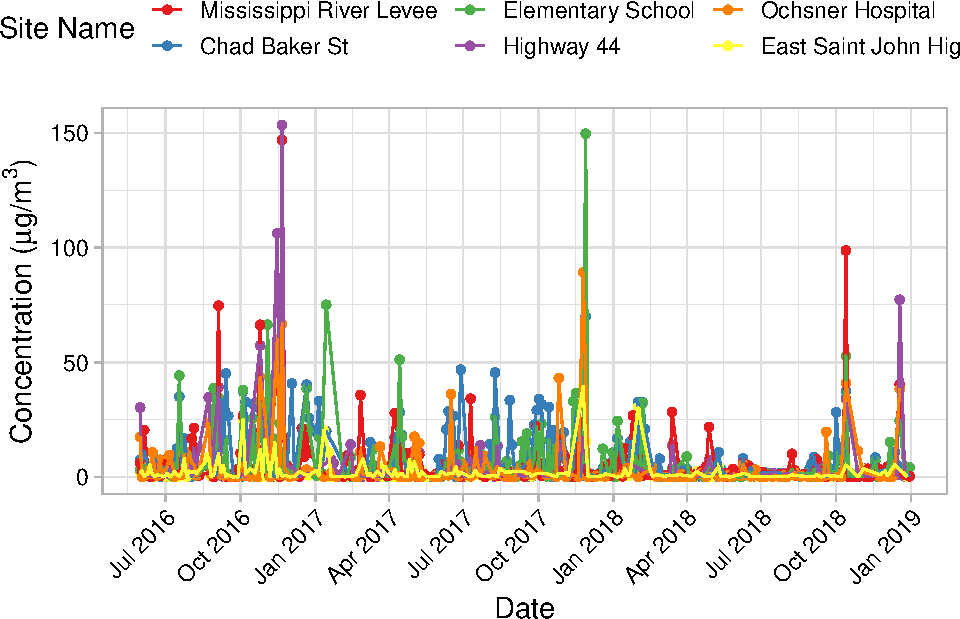
\includegraphics{Li_ENV872_Project_files/figure-latex/unnamed-chunk-2-1.pdf}
\caption{Chloroprene concentrations at six monitoring sites over time}
\end{figure}

\begin{figure}
\centering
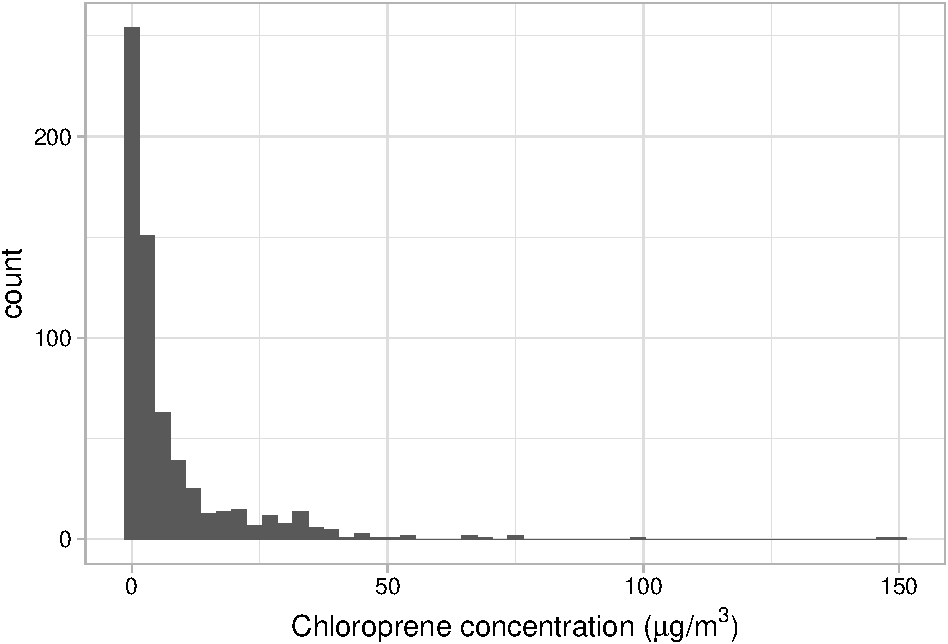
\includegraphics{Li_ENV872_Project_files/figure-latex/unnamed-chunk-3-1.pdf}
\caption{Distribution of chloroprene concentration}
\end{figure}

\begin{figure}
\centering
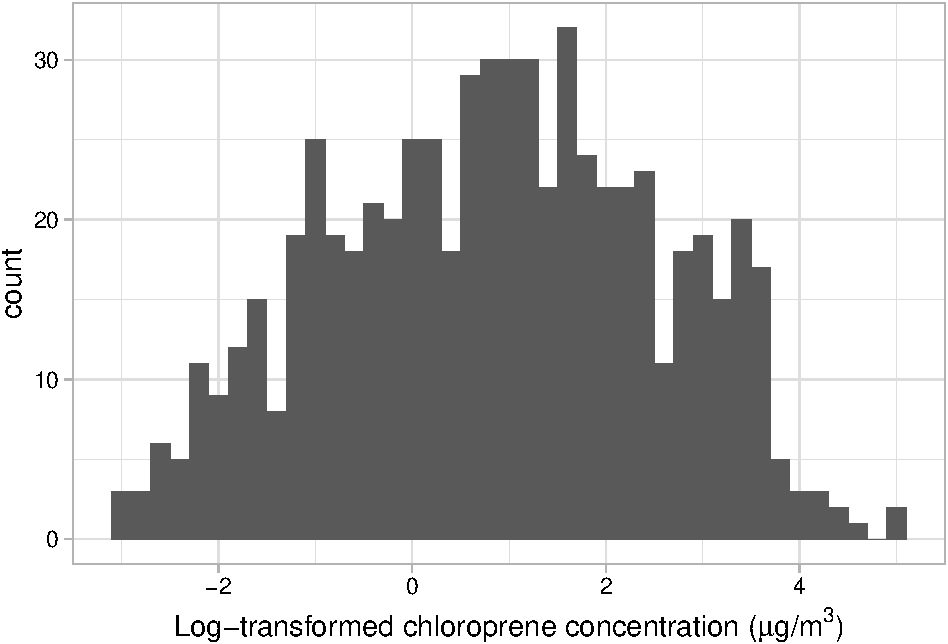
\includegraphics{Li_ENV872_Project_files/figure-latex/unnamed-chunk-4-1.pdf}
\caption{Distribution of log-transformed chloroprene concentration}
\end{figure}

\newpage

\section{Analysis}\label{analysis}

We begin with testing the normality of the chloroprene concentrations.

\begin{Shaded}
\begin{Highlighting}[]
\CommentTok{# Distribution test}
\CommentTok{# Normal distribution}
\KeywordTok{shapiro.test}\NormalTok{(data.near.gather}\OperatorTok{$}\NormalTok{Concentration)}
\end{Highlighting}
\end{Shaded}

\begin{verbatim}
## 
##  Shapiro-Wilk normality test
## 
## data:  data.near.gather$Concentration
## W = 0.54291, p-value < 2.2e-16
\end{verbatim}

\begin{Shaded}
\begin{Highlighting}[]
\KeywordTok{shapiro.test}\NormalTok{(data.near.gather}\OperatorTok{$}\NormalTok{Log.concentration)}
\end{Highlighting}
\end{Shaded}

\begin{verbatim}
## 
##  Shapiro-Wilk normality test
## 
## data:  data.near.gather$Log.concentration
## W = 0.98788, p-value = 3.678e-05
\end{verbatim}

Even though the results of Shapiro test show that neither of the
original or log-transformed chloroprene concentrations is normally
distributed, considering the nature of this dataset and the distribution
figures above, we performed the generalized linear model using the
log-transformed data. And the result shows that there is a statistically
significant correlation between wind speed and chloroprene concentrtion
(Generalized linear model; coefficient = -0.303, t-value = -4.940, p
\textless{} 0.0001). The correlation is shown in Figure 4.

\begin{Shaded}
\begin{Highlighting}[]
\NormalTok{speed.glm <-}\StringTok{ }\KeywordTok{glm}\NormalTok{(}\DataTypeTok{data =}\NormalTok{ data.near.gather, Log.concentration }\OperatorTok{~}\StringTok{ }\NormalTok{Wind.Speed)}
\KeywordTok{summary}\NormalTok{(speed.glm)}
\end{Highlighting}
\end{Shaded}

\begin{verbatim}
## 
## Call:
## glm(formula = Log.concentration ~ Wind.Speed, data = data.near.gather)
## 
## Deviance Residuals: 
##     Min       1Q   Median       3Q      Max  
## -4.0957  -1.1894  -0.0421   1.2365   4.0764  
## 
## Coefficients:
##             Estimate Std. Error t value Pr(>|t|)    
## (Intercept)  1.71967    0.18806   9.144  < 2e-16 ***
## Wind.Speed  -0.30294    0.06132  -4.940 9.96e-07 ***
## ---
## Signif. codes:  0 '***' 0.001 '**' 0.01 '*' 0.05 '.' 0.1 ' ' 1
## 
## (Dispersion parameter for gaussian family taken to be 2.749833)
## 
##     Null deviance: 1827.0  on 641  degrees of freedom
## Residual deviance: 1759.9  on 640  degrees of freedom
## AIC: 2475.3
## 
## Number of Fisher Scoring iterations: 2
\end{verbatim}

\begin{figure}
\centering
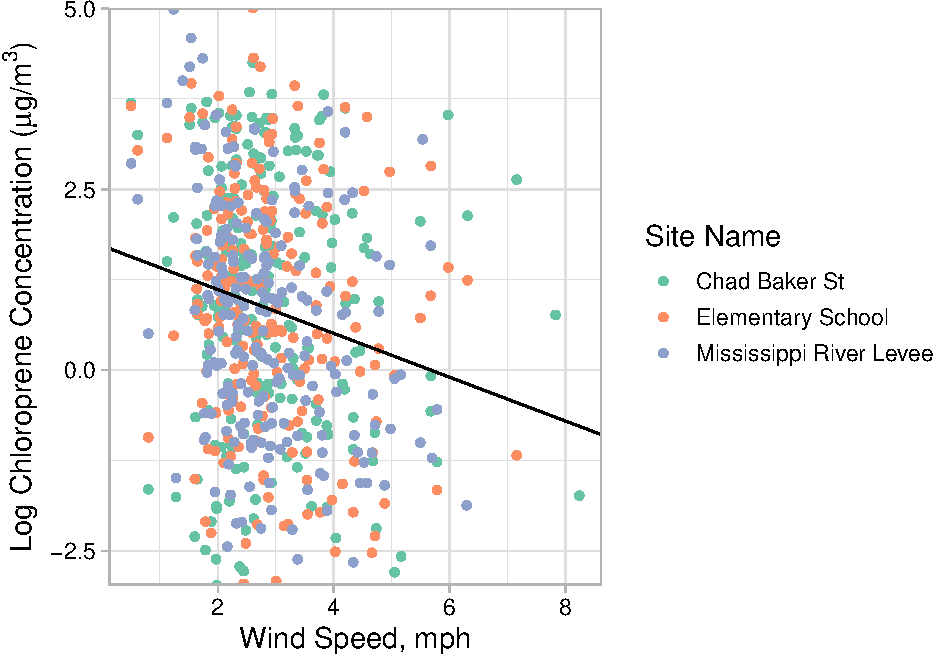
\includegraphics{Li_ENV872_Project_files/figure-latex/unnamed-chunk-7-1.pdf}
\caption{Chloroprene concentration and wind speed}
\end{figure}

Another objective of this project is to investigate the change of
chloroprene concentrations over time. As shown in Table 2, there is an
obvious drop in chloroprene concentrations from 2016 to 2018. The result
of ANOVA test also suggests that the concentrations are statistically
significant different from each other in 2016, 2017, and 2018 (ANOVA
test; F-statistic = 19.76, df = 1155, p-value \textless{} 0.0001).

Pettitt's test allows us to find the changing point in our data.
According to Denka, the emission reduction projects were implemented by
the company to reduce chloroprene emissions around the beginning in
2018. As the results shown below, the changing points occurred on
2017-11-13 at Chad Baker St, on 2018-01-15 at Fifth Ward Elementary
School, and on 2018-01-09 at Missippi River Levee, which agree with the
statement of the company.

\begin{Shaded}
\begin{Highlighting}[]
\CommentTok{# Test for change over time}
\NormalTok{Year.mean <-}\StringTok{ }\NormalTok{data.gather }\OperatorTok
\StringTok{  }\KeywordTok{filter}\NormalTok{(}\OperatorTok{!}\KeywordTok{is.na}\NormalTok{(Concentration)) }\OperatorTok
\StringTok{  }\KeywordTok{group_by}\NormalTok{(Year) }\OperatorTok
\StringTok{  }\KeywordTok{summarize}\NormalTok{(}\StringTok{"Mean"}\NormalTok{ =}\StringTok{ }\KeywordTok{mean}\NormalTok{(Concentration))}
\KeywordTok{kable}\NormalTok{(Year.mean, }\DataTypeTok{caption =} \StringTok{"Annual average of chloroprene concentration"}\NormalTok{)}
\end{Highlighting}
\end{Shaded}

\begin{longtable}[]{@{}rr@{}}
\caption{Annual average of chloroprene concentration}\tabularnewline
\toprule
Year & Mean\tabularnewline
\midrule
\endfirsthead
\toprule
Year & Mean\tabularnewline
\midrule
\endhead
2016 & 9.986195\tabularnewline
2017 & 6.154984\tabularnewline
2018 & 3.659313\tabularnewline
\bottomrule
\end{longtable}

\begin{Shaded}
\begin{Highlighting}[]
\NormalTok{air.lm <-}\StringTok{ }\KeywordTok{aov}\NormalTok{(}\DataTypeTok{data =}\NormalTok{ data.gather,  Concentration }\OperatorTok{~}\StringTok{ }\KeywordTok{as.factor}\NormalTok{(Year))}
\KeywordTok{summary}\NormalTok{(air.lm)}
\end{Highlighting}
\end{Shaded}

\begin{verbatim}
##                   Df Sum Sq Mean Sq F value   Pr(>F)    
## as.factor(Year)    2   7012    3506   19.76 3.65e-09 ***
## Residuals       1155 204943     177                     
## ---
## Signif. codes:  0 '***' 0.001 '**' 0.01 '*' 0.05 '.' 0.1 ' ' 1
\end{verbatim}

\begin{Shaded}
\begin{Highlighting}[]
\CommentTok{# Test for change point}
\CommentTok{# Remove NAs}
\NormalTok{data.clean <-}\StringTok{ }\KeywordTok{na.exclude}\NormalTok{(data.all)}
\CommentTok{# Pettitt test}
\KeywordTok{pettitt.test}\NormalTok{(data.clean}\OperatorTok{$}\NormalTok{Chad.Baker)}
\end{Highlighting}
\end{Shaded}

\begin{verbatim}
## 
##  Pettitt's test for single change-point detection
## 
## data:  data.clean$Chad.Baker
## U* = 6044, p-value = 0.0004784
## alternative hypothesis: two.sided
## sample estimates:
## probable change point at time K 
##                             174
\end{verbatim}

\begin{Shaded}
\begin{Highlighting}[]
\KeywordTok{pettitt.test}\NormalTok{(data.clean}\OperatorTok{$}\NormalTok{Elementary.School)}
\end{Highlighting}
\end{Shaded}

\begin{verbatim}
## 
##  Pettitt's test for single change-point detection
## 
## data:  data.clean$Elementary.School
## U* = 5878, p-value = 0.0007516
## alternative hypothesis: two.sided
## sample estimates:
## probable change point at time K 
##                             195
\end{verbatim}

\begin{Shaded}
\begin{Highlighting}[]
\KeywordTok{pettitt.test}\NormalTok{(data.clean}\OperatorTok{$}\NormalTok{Levee)}
\end{Highlighting}
\end{Shaded}

\begin{verbatim}
## 
##  Pettitt's test for single change-point detection
## 
## data:  data.clean$Levee
## U* = 4782, p-value = 0.01082
## alternative hypothesis: two.sided
## sample estimates:
## probable change point at time K 
##                             193
\end{verbatim}

\begin{figure}
\centering
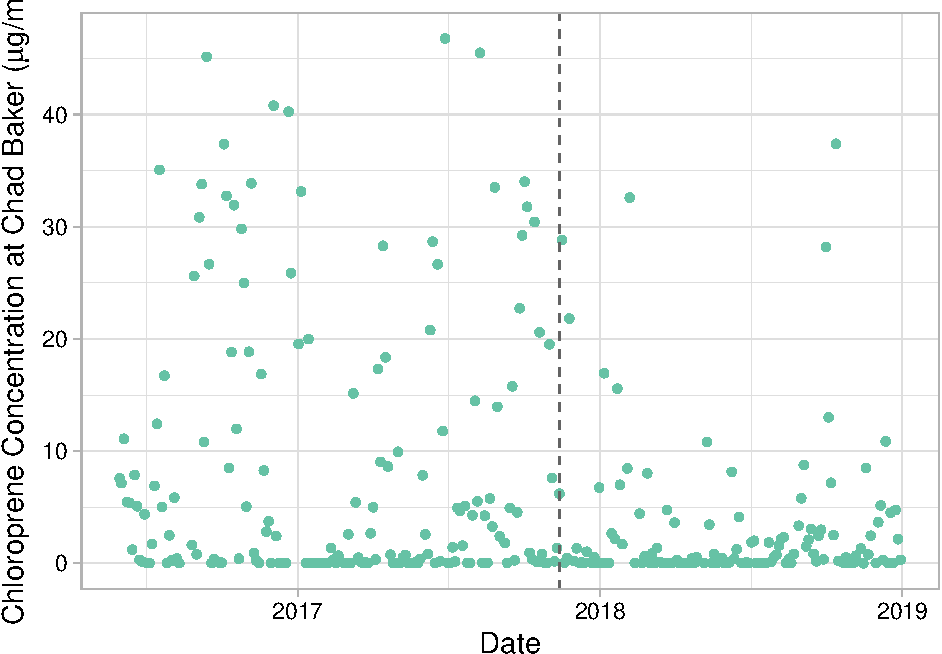
\includegraphics{Li_ENV872_Project_files/figure-latex/unnamed-chunk-9-1.pdf}
\caption{Chloroprene change point at Chade Baker St}
\end{figure}

\begin{figure}
\centering
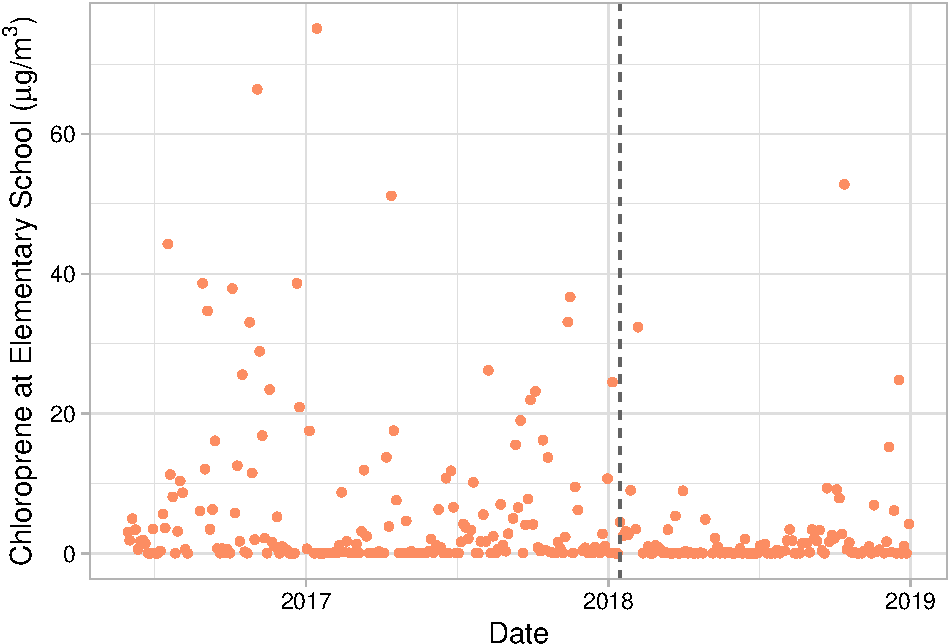
\includegraphics{Li_ENV872_Project_files/figure-latex/unnamed-chunk-10-1.pdf}
\caption{Chloroprene change point at Elementary School}
\end{figure}

\begin{figure}
\centering
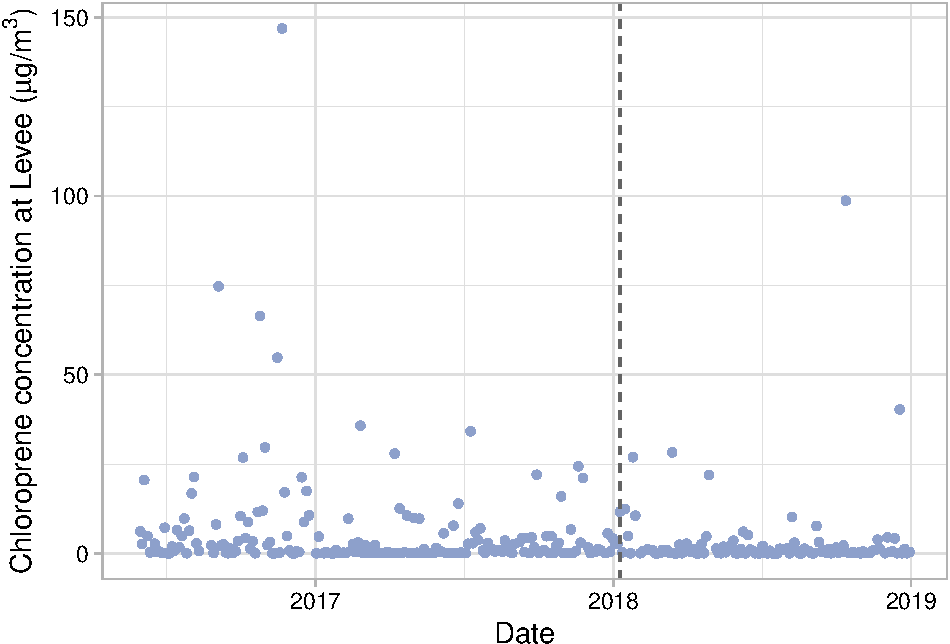
\includegraphics{Li_ENV872_Project_files/figure-latex/unnamed-chunk-11-1.pdf}
\caption{Chloroprene change point at Mississippi River Levee}
\end{figure}

\newpage

\section{Summary and Conclusions}\label{summary-and-conclusions}

The results show that there is a statistically significant negative
correlation between chloroprene concentration and wind speed at the
three monitoring sites within 1 km to the Denka facility. Residents
living close to the Denka facility are facing high risk of developing
cancer because of potential explosure of chloroprene. Meteorology
factors may play an essential part in the distribution of chloroprene.
The results of the project suggests that wind speed affacts the
concentrations of chloroprene close to the facility.

Chloroprene concentrations decline significantly from 2016 to 2018, and
the changing points at the three monitoring sites within 1 km to the
facility all occurred around January 2018, which is accordant with the
implementation time of the emission reduction projects announced by
Denka. Substantial decreases in chloropren concentraitons have been seen
from 2016 to 2018. However, the current concentrations still far exceed
the recommended level without increasing risk of cancer (0.2
µg/m\textsuperscript{3}). More efforts need to be made to protect public
health in the LaPlace community.


\end{document}
